\documentclass[12pt, a4paper]{article}
\renewcommand*\contentsname{Inhaltsverzeichnis}
\usepackage[ngerman]{babel}
\usepackage{mathptmx}
\usepackage{blindtext}
\usepackage{emptypage}
\usepackage{wrapfig}
\usepackage[pdftex]{graphicx}
\usepackage{geometry}
\usepackage{setspace}
\usepackage[version=4,arrows=pgf-filled,
textfontname=sffamily,
mathfontname=mathsf]{mhchem}
\usepackage{mathcomp}
\usepackage{multirow}
\usepackage[table]{xcolor}
\usepackage{array}
\usepackage{hyperref}
\usepackage{csquotes}
\usepackage[backend=biber,style=chem-acs,articletitle=true,sorting=none]{biblatex}
\addbibresource{literatur.bib}  % Deine .bib-Datei einbinden
\renewcommand{\arraystretch}{1.3}
\DeclareCiteCommand{\cite}
  {\usebibmacro{prenote}}
  {\textsuperscript{\printfield{labelnumber}}}
  {\multicitedelim}
  {\usebibmacro{postnote}}


 \geometry{
 a4paper,
 total={170mm,257mm},
 left=25mm,
 top=25mm,
 }
\setstretch{1.213}


\newcommand{\datum}{\day.\month.\year}
\DeclareGraphicsExtensions{.pdf,.jpeg,.png,.jpg} 

\begin{document}


\begin{figure}
    \includegraphics[scale=0.14]{Universität_Bayreuth.svg.png}
\end{figure}


%Deckblatt

{\raggedright Universität Bayreuth\\  95447 Bayreuth}


\vspace{5cm}

\begin{center}
{\LARGE\bf{Anorganische Chemie III}} \\  
\vspace{1cm}
{\Large\bf{Ferroelektrika}}\\
\vspace{0.5cm}
{\large Justus Friedrich\\}
{Studiengang: B.Sc. Chemie\\}
{4. Fachsemester}
\end{center}





\thispagestyle{empty}
\begin{center}
{\small Matrikelnummer: 1956010 \\
E–Mail:  bt725206@myubt.de}
\end{center}

\vspace{5cm}

\begin{center}
  \today
\end{center}


\newpage
%Inhaltsverzeichnis
\tableofcontents
\thispagestyle{empty}


%Teil 1
\newpage
\setcounter{page}{1}
\section{Einleitung}



\subsection{Einführung}
Ferroelektrikuas sind besonders in den letzten 10 Jahren interessanter geworden, 
das liegt an den möglichen Anwendungen eines Ferroelektrikas. Diese können mit einem kurzen 
externen elektrischen Feld polarisiert werden, und behalten diese Polarisation auch nach dem Abschalten 
des elktrischen Feldes bei. Somit können sie zu einem Nichtflüchtiger Speicher verwendet werden.\cite{Damjanovic.1998}


\subsection{Ziel des Versuchs}
{
In Versuch soll $SrTiO_3$ und $BaTiO_3$ hergestellt werden. Dabei wird die Probe zweimal geglüht, nach dem erstem
und dem zweiten Mal glühen wird jeweils ein Pulverdiffraktogramm aufgenommen. Daraus soll dann die Halbwertsbreite und 
der Goldschmidtfaktor bestimmt werden. Außerdem werden die Unterschiede zwischen den Kristallsystemen von $SrTiO_3$ und $BaTiO_3$ 
untersucht. Zudem soll die Probe des $BaTiO_3$ mit der einer phasenreinen Probe von $BaTiO_3$ verglichen werden.\cite{Skript}
}

\subsection{Zusatzfragen}
Festkörperreaktionen verlaufen extrem Langsam, da die einzelen Stoffe nazu garnicht ineinader Diffundieren können. Dass führt 
dazu, dass die Reaktanden miteinader kaum Kontakt habe. Um eine gute Ausbeute zu erhalten, wird in der Regel die Reaktanden oft gemörsert, dann gepresst und 
erhitzt. Dieser Vorgang wird solange Wiederholt bis die Ausbeute Ausrreichend hoch ist.\\
\ce{BaCO3} wird als Edukt vermieden, da dieses sehr schlecht Löslich ist. Da in dieser Arbeitsvorschrift zunächst die Reaktanden mit Aceton verrieben wird, lässt sich durch eine 
höhre Löslichkeit eine bessere Vermischung erzielen. Daher wird \ce{Ba(CH3COO)2} eingesetzt, welches in Ofen dann zu \ce{BaCO3} zerfällt. 



\newpage
%Teil2
\section{\texorpdfstring{Synthese von $SrTiO_3$ und $BaTiO_3$}{Synthese von SrTiO3 und BaTiO3}}
\subsection{\texorpdfstring{Synthese von $SrTiO_3$}{Synthese von SrTiO3}}
{Es werden 2.95 g (20 mmol) von $SrCO_3$ mit 1.60 g (20 mmol) $TiO_2$ in einem Mörser gegeben. 
Dazu wird etwas Aceton gegeben und 
zu einem homogenen Brei vermengt. Dafür sind ca. 10 Min nötig. Nachdem das Aceton vollstädig verdampft ist, wird mit dem Pulver eine 300 mg 
Tablette bei 10 Tonnen gepresst. Die Tablette wird daraufhin in einem Tiegel für 6h bei 600 °C geglüht.\\
Am Nächten Tag wird die Tablette gemörsert und etwas Pulver für ein Pulverdiffraktogramm entnommen. Danach wird erneut eine Tablette gepresst und über Nacht
bei 1000 °C geglüht. Dabei wird der Ofen mit 6 $\frac{\tccentigrade}{min}$ geheizt. Nach dem Glühen wird der Wird erneut ein Pulverdiffraktogramm aufgenommen.
}
\subsection{\texorpdfstring{Synthese von $BaTiO_3$}{Synthese von BaTiO3}}
{
Es werden 2.55 g (10 mmol) von $Ba(CH_3COO)_2$ mit 0.80 g (10 mmol) $TiO_2$ in einem Mörser gegeben.
Dazu wird etwas Aceton gegeben und 
zu einem homogenen Brei vermengt. Dafür sind ca. 10 Min nötig. Nachdem das Aceton vollstädig verdampft ist, wird mit dem Pulver eine 300 mg 
Tablette bei 10 Tonnen gepresst. Die Tablette wird daraufhin in einem Tiegel für 6h bei 600 °C geglüht.\\
Am Nächten Tag wird die Tablette gemörsert und etwas Pulver für ein Pulverdiffraktogramm entnommen. Danach wird erneut eine Tablette gepresst und über Nacht
bei 1000 °C geglüht. Dabei wird der Ofen mit 6 $\frac{\tccentigrade}{min}$ geheizt. Nach dem Glühen wird der Wird erneut ein Pulverdiffraktogramm aufgenommen.
}
\subsection{Reaktionsgleichungen }
\begin{center}
\ce{SrCO3 + TiO2 -> SrTiO3 +CO2}\\
\ce{Ba(CH3COO)2 -> BaC2O4 -> BaCO3} Quelle\cite{Reaktionsgleichungen}\\
\ce{BaCO3 + TiO2 -> BaTiO3 +CO2} Quelle\cite{Reaktionsgleichungen}


\end{center}
\newpage
\section{Auswertung}
\subsection{Phasenanalyse}
\subsubsection{\texorpdfstring{Phasenanalyse von \ce{SrTiO3}}{Phasenanalyse von SrTiO3}}
Die XRD-Probe, die nach dem erstem Mal Tempern aufgenommen wurde, besteht primär noch aus den Edukten. 
Die Phasenanalyse, im Programm HighScore Plus, ergab mit einem Score von 64 eine primäre Phase von \ce{TiO2} mit dem Referenzcode 01-084-1285.
Die sekundäre Phase mit einem Score von 58 ist \ce{SrCO3} (Referenzcode 00-005-0418). Das eigentliche Produkt \ce{SrTiO3} liegt in der Probe
kaum vor, der Score ist nur 1 mit dem Referenzcode 00-001-1018. Die benutzten XRD-Reflexe sind in \mbox{Abbildung \ref{Ferro1SrTiO3}} dargestellt, und die Probe wurde vom Platz 20 hergestellt.


\begin{figure}[h!]
  \begin{center}
   
  \includegraphics[scale=0.5]{Ferro1SrTiO3.png}
\caption{\textit{XRD-Messung von einer Mischung aus \ce{SrCO3} und \ce{TiO2} die für 6h bei 600°C getempert wurde. Außerdem sind Referenzreflexe von 
\ce{SrCO3} (Referenzcode 00-005-0418) und \ce{TiO2} (Referenzcode 01-084-1285) abgebildet.}}

\label{Ferro1SrTiO3}

 \end{center}

\end{figure}
\noindent
Anschließend wurde die Probe gemörsert und erneut gepresst und 1000 °C für 8h getempert. Die danach durchgeführte
XRD-Messung ergab dass das Produkt \ce{SrTiO3} (Referenzcode 01-079-0174) einen Score von 97 besitzt. Somit ist das Produkt zum Großteil in der Probe. 
Allerdings ist auch \ce{TiO2} (Referenzcode 01-073-1581) zu finden. Diese Phase hat einen Score von 8. Die Abbildung \ref{Ferro2SrTiO3} zeigt die XRD-Reflexe. Die Probe ist wieder von Platz 20.
\newpage

\begin{figure}[!h]
  \begin{center}
   
  \includegraphics[scale=0.5]{Ferro2SrTiO3.png}
\caption{\textit{XRD-Messung von \ce{SrTiO3} mit \ce{TiO2} Verunreinigungen. Außerdem sind Referenzreflexe von 
\ce{SrTiO3} (Referenzcode 01-079-0174) und \ce{TiO2} (Referenzcode 01-073-1581) abgebildet.}}
\label{Ferro2SrTiO3}
 \end{center}
\end{figure}
\noindent
Anschließend wird die Elementarzelle von hergestellten \ce{SrTiO3} untersucht und mit der Referenz verglichen. Dies wird in der Tabelle \ref{Kastenlängeferrosrtio3} dargestellt.

\begin{table}[h!]
\caption{\textit{Zeigt die Theoretische und Festgestellte Einheitszelle von den hergestellten \ce{SrTiO3} (Referenzcode 01-079-0174). Die Verfeinerung wurde mithilfe des Programmes HighScore Plus durchgeführt. }}
\begin{center}
\begin{tabular}{|>{\columncolor{lime}}p{4cm}|>{\centering\arraybackslash}p{4cm}|>{\centering\arraybackslash}p{4cm}|}
   \hline
   \rowcolor{gray}
   &Theoretische Elementarzelle& Festgestellte Elementarzelle (Standardabweichung) \\
   \hline
   a[\AA]&3.9050& 3.9048(4)\\
   \hline
   b[\AA]&3.9050& 3.9048(4)\\
   \hline
   c[\AA]&3.9050& 3.9048(4)\\
   \hline
   $\alpha$[°]&90& 90\\
   \hline
   $\beta$[°]&90& 90\\
   \hline
   $\gamma$[°]&90& 90\\
   \hline
   Volumen[\AA$^3$]&59.55 & 59.54\\
   \hline

\end{tabular}
\label{Kastenlängeferrosrtio3}
\end{center}
\end{table}

\noindent
Die Festgestellten Werte der Einheitszelle weichen nur geringfügig von der Theoretischen Einheitszelle ab, somit war die Synthese des 
 \ce{SrTiO3} ein Erfolg.

\newpage
\subsubsection{\texorpdfstring{Phasenanalyse von \ce{BaTiO3}}{Phasenanalyse von BaTiO3}}
Die XRD-Probe zeigt, dass das gesamte \ce{Ba(CH3COO)2}, nach dem ersten Mal Tempern, in \ce{BaCO3} umgewandelt wurde.
Dieses besitzt zum Referenzreflex (00-005-0378) einen Score von 61. Zudem zeigt sich, das die 
Festkörperreaktion schon gestartet ist, da mit einen Score von 12 und $4\% $ schon \ce{BaTiO3} (Referenzcode 01-075-0460) vorliegt.
Außerdem lässt sich die Phase von \ce{TiO2} (Referenzcode 01-084-1285) feststellen. Die XRD-Messung und die Referenzreflexe sind in der Abbildung \ref{Ferro1BaTiO3}
abgebildet. Die Probe stammt von Platz 25.

\begin{figure}[!h]
  \begin{center}
   
  \includegraphics[scale=0.5]{Ferro1BaTiO3.png}
\caption{\textit{XRD-Messung von \ce{BaCO3} mit \ce{TiO2} und \ce{BaTiO3}. Außerdem sind Referenzreflexe von 
\ce{BaCO3} (Referenzcode 00-005-0378), \ce{TiO2} (Referenzcode 01-084-1285) und \ce{BaTiO3} (Referenzcode 01-075-0460) abgebildet.}}
\label{Ferro1BaTiO3}
 \end{center}
\end{figure}

\noindent
Nach dem zweiten mal Tempern, lässt sich nur noch \ce{BaTiO3} (Referenzcode 01-083-1876) feststellen. Allerdings lässt sich zwei 
verschiedene Strukturen von den \ce{BaTiO3} feststellen. Einmal in der orthorhombische Anordnung mit 27\% (Referenzcode 01-075-1608; Score 62) und 
in der Tetragonale Anordnung mit 73\% (Referenzcode 01-083-1876; Score 87). Weitere Phasen wurden nicht festgestellt. Die XRD-Messung und die Referenzreflexe sind in
der Abbildung \ref{Ferro2BaTiO3} abgebildet. Die Probe stammt von Platz 25.
\newpage

\begin{figure}[!h]
  \begin{center}
   
  \includegraphics[scale=0.5]{Ferro2BaTiO3.png}
\caption{\textit{XRD-Messung von orthorhombischen \ce{BaTiO3} und tetragonalen \ce{BaTiO3}. Außerdem sind Referenzreflexe von 
orthorhombischen \ce{BaTiO3} (Referenzcode 01-075-1608) und tetragonalen \ce{BaTiO3} (Referenzcode 01-083-1876) abgebildet.}}
\label{Ferro2BaTiO3}
 \end{center}
\end{figure}
\noindent
Anschließend wird die Elementarzelle von tetragonalen \ce{BaTiO3} bestimmt, da dies die Hauptphase ist. Und mit der Referenz verglichen, dies wird in Tabelle \ref{Kastenlängeferrobatio3} dargestellt.

\begin{table}[h!]
\caption{\textit{Zeigt die Theoretische und Festgestellte Einheitszelle von den hergestellten \ce{BaTiO3} (Referenzcode 01-083-1876). Die Verfeinerung wurde mithilfe des Programmes HighScore Plus durchgeführt. }}
\begin{center}
\begin{tabular}{|>{\columncolor{lime}}p{4cm}|>{\centering\arraybackslash}p{4cm}|>{\centering\arraybackslash}p{4cm}|}
   \hline
   \rowcolor{gray}
   &Theoretische Elementarzelle& Festgestellte Elementarzelle (Standardabweichung) \\
   \hline
   a[\AA]&\centering{3.99450}& 3.998 (1)\\
   \hline
   b[\AA]&3.99450& 3.998 (1)\\
   \hline
   c[\AA]&4.03350& 4.021 (3)\\
   \hline
   $\alpha$[°]&90& 90\\
   \hline
   $\beta$[°]&90& 90\\
   \hline
   $\gamma$[°]&90& 90\\
   \hline
   Volumen[\AA$^3$]&64.36 & 64.28\\
   \hline

\end{tabular}
\label{Kastenlängeferrobatio3}
\end{center}
\end{table}
\noindent
Die Festgestellten Werte der Einheitszelle weichen nur minimal von der Referenz ab. Somit war auch die Synthes des \ce{BaTiO3} ein Erfolg.
\newpage
\subsection{Scherrer-Formel}
Um die Korngröße der Kristallinen Struktur zu bestimmen, 
kann die Scherrer-Formel hergenommen werden. 

\begin{equation}
  L=\frac{K\lambda}{\Delta H(2\theta)cos(\theta)}
\end{equation}
\noindent
Dabei ist $L$ die Kristallitgröße, $K$ eine Konstante, die von Kristallsystem abhänig ist, $\Delta H(2\theta)$ ist die Halbwertsbreite der  Beugungslinien des 111 Reflex 
in Bogenmaß und $\lambda$ ist die Wellenlänge der Röngtenstrahlung. Die Werte der Berechnung sind in Tabelle \ref{Scherrer} aufgelistet.

\begin{table}[h!]
  \caption{\textit{Die Tabelle zeigt die Lage und Halbwertsbreiten des 111 Reflex von \ce{BaTiO3} und \ce{SrTiO3}, die daraus berechnete Kristalitgröße. Zudem wird zwischen den ersten und Zweiten Tempern verglichen. }}
  \begin{center}
    \begin{tabular}{|>{\columncolor{lime}}p{5.3cm}|>{\centering\arraybackslash}p{2.3cm}|>{\centering\arraybackslash}p{2.3cm}|>{\centering\arraybackslash}p{2.3cm}|>{\centering\arraybackslash}p{2.3cm}|}
      \hline
      \rowcolor{gray}
      &\ce{SrTiO3} \mbox{1. Tempern} & \ce{SrTiO3} \mbox{2. Tempern} & \ce{BaTiO3} \mbox{1. Tempern} & \ce{BaTiO3} \mbox{2. Tempern}\\
\hline
Lage [$2\theta$]&39.903&39.952°&37.868&38.909°\\
\hline
Halbwertsbreite in Bogenmaß&1.005$\cdot 10^{-2}$&2.652$\cdot 10^{-3}$&7.539$\cdot 10^{-3}$&2.199$\cdot 10^{-3}$\\
\hline
Kristalitgröße [\AA]&188&713&237&847\\
\hline
    \end{tabular}
    \label{Scherrer}
  \end{center}
\end{table}
\noindent
Aus der Tabelle \ref{Scherrer} lässt sich ablesen, dass beim Zweiten Tempern die Kristalitgröße nochmal Stark anwächst. Das leigt an den generell höheren Umsatz 
der Reaktanden. Außerdem 
lässt sich ablesen, dass \ce{BaTiO3} generell größere Kristalle bildet als \ce{SrTiO3}.


\subsection{Goldschmidtfaktor}
Der Goldschmidtfaktor gibt an wie gut eine Elementarzelle sich gegenüber einer perfekt kubischen Anordnung verhält. Er wird durch Gleichung 2 berechnet.
\begin{equation}
  t=\frac{d_{A-O}}{\sqrt{2}\cdot d_{B-O}}=\frac{\sqrt{(\frac{1}{2}a)^2+(\frac{1}{2}b)^2}}{\sqrt{2}\cdot \frac{1}{2}c}
\end{equation}
Die Werte für die berechnung und der Goldschmidtfaktor wird in der Tabelle \ref{Goldschmidt} angegeben. 
\begin{table}[h!]
  \begin{center}
    
  
  \caption{\textit{Tabelle zeigt die Werte für $d_{A-O}$, $d_{B-O}$, sowie den Goldschmitfaktor $t$ für \ce{SrTiO3} und \ce{BaTiO3}}}
\begin{tabular}{|>{\columncolor{lime}}p{4cm}|>{\centering\arraybackslash}p{4cm}|>{\centering\arraybackslash}p{4cm}|}
  \hline
  \rowcolor{gray}
  &\ce{SrTiO3}&\ce{BaTiO3}\\
  \hline
  $d_{A-O}$&2.757&2.827\\
  \hline
  $d_{B-O}$&1.9495&2.0105\\
  \hline
  $t$&1&0.994\\
  \hline
\end{tabular}
\label{Goldschmidt}
\end{center}
  
\end{table}
\\
\noindent
Aufgrund des Goldschmidtfaktors lässt sich darauf schließen, das \ce{SrTiO3} eine perfekte kubische Perowskit-Struktur aufweißt.
\ce{BaTiO3} weißt allerdings ein Faktor von 0.994 auf, dies weißt auf einen leichten defekt in der Kristallstruktur hin. 
Welche dadurch kommt, dass die Barium-Atome zu Groß sind, um in die Kristallstruktur zu passen. 
Dennoch sind beide Strukturen stabil.\cite{Skript} 

\subsection{\texorpdfstring{Vergleich der Kristallstruktur von \ce{BaTiO3} bei 293 K und 400 K}{Vergleich der Kristallstruktur von BaTiO3 bei 293 K und 400 K}}

Es werden von einer Reinen \ce{BaTiO3}-Probe zwei XRD-Messungen aufgenommen. Dabei wird die Temperatur variert. Die eine Messung wird 
bei 293 K durchgeführt, und die andere bei 400 K.

\begin{figure}[h!]
  \begin{center}
    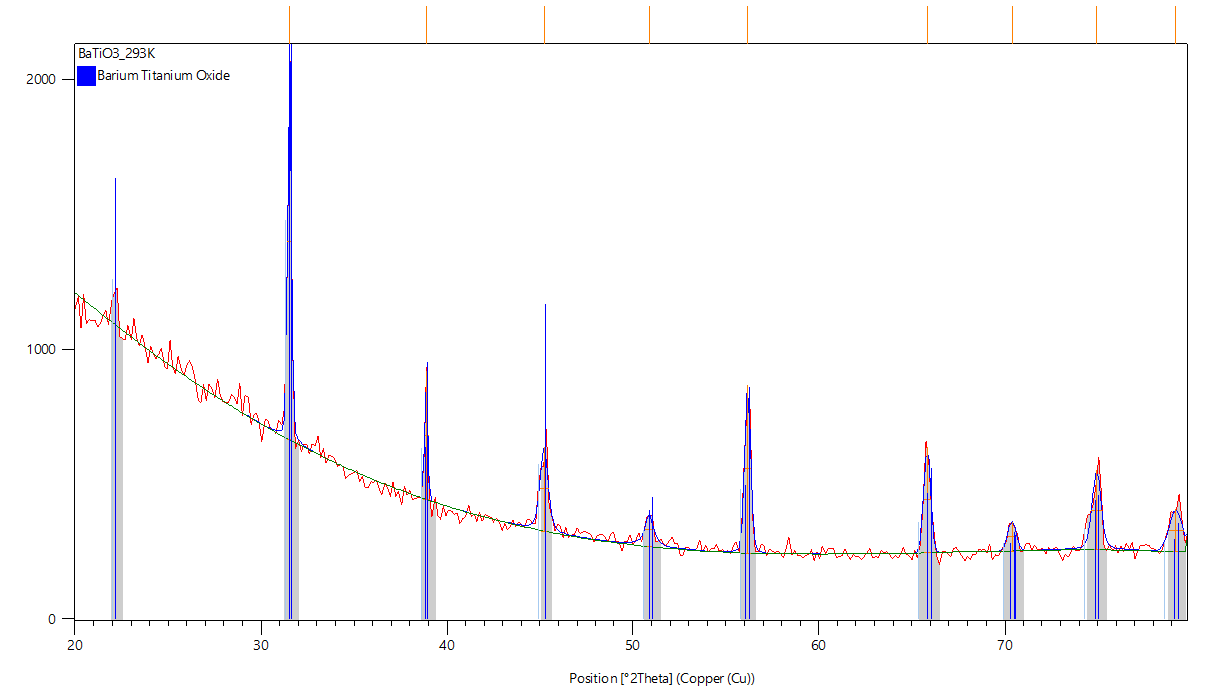
\includegraphics[scale=0.5]{BaTiO3293.png}
  \end{center}
\caption{Zeigt die XRD-Reflexe von reinen \ce{BaTiO3} bei 293 K, mit Referenzreflexen von rhomboedrischen \ce{BaTiO3} (Referenzcode 01-085-1790).}
\label{BaTiO3293}
\end{figure}
\noindent
Aus der Abbildung \ref{BaTiO3293} lässt sich schließen, dass reinens \ce{BaTiO3} bei 20 °C (293.15 K) nazu nur in einer 
rhomboedrischen Struktur vorliegt (Referenzcode 01-085-1790; Score 86; 95\%). Ca 5\% des \ce{BaTiO3} (Referenzcode 01-075-0213)liegt in einer Kubischen Struktur vor. Die Strucktur der 
Festgestellte Verfeinerten Elementarzelle und der Referenz wird in der Tabelle \ref{Kastenlängebatio3293} dargestellt.

\begin{table}
\caption{\textit{Zeigt die Theoretische und Festgestellte Einheitszelle von den hergestellten \ce{BaTiO3} (Referenzcode 01-083-1876). Die Verfeinerung wurde mithilfe des Programmes HighScore Plus durchgeführt. }}
\begin{center}
\begin{tabular}{|>{\columncolor{lime}}p{4cm}|>{\centering\arraybackslash}p{4cm}|>{\centering\arraybackslash}p{4cm}|}
   \hline
   \rowcolor{gray}
   &Theoretische Elementarzelle& Festgestellte Elementarzelle (Standardabweichung) \\
   \hline
   a[\AA]&\centering{5.653990}& 5.670(2) \\
   \hline
   b[\AA]&5.653990& 5.670(2)\\
   \hline
   c[\AA]&6.953900& 6.936(4)\\
   \hline
   $\alpha$[°]&90& 90\\
   \hline
   $\beta$[°]&90& 90\\
   \hline
   $\gamma$[°]&120& 120\\
   \hline
   Volumen[\AA$^3$]&192.52 & 193.09\\
   \hline

\end{tabular}
\label{Kastenlängebatio3293}
\end{center}
\end{table}
\newpage
\noindent
Anschließend wird die Struktur von \ce{BaTiO3} bei 400K betrachtet. Die gemessenen XRD-Reflexe sind in der Abbildung \ref{BaTiO3400} dargestellt.
\begin{figure}[h!]
  \begin{center}
    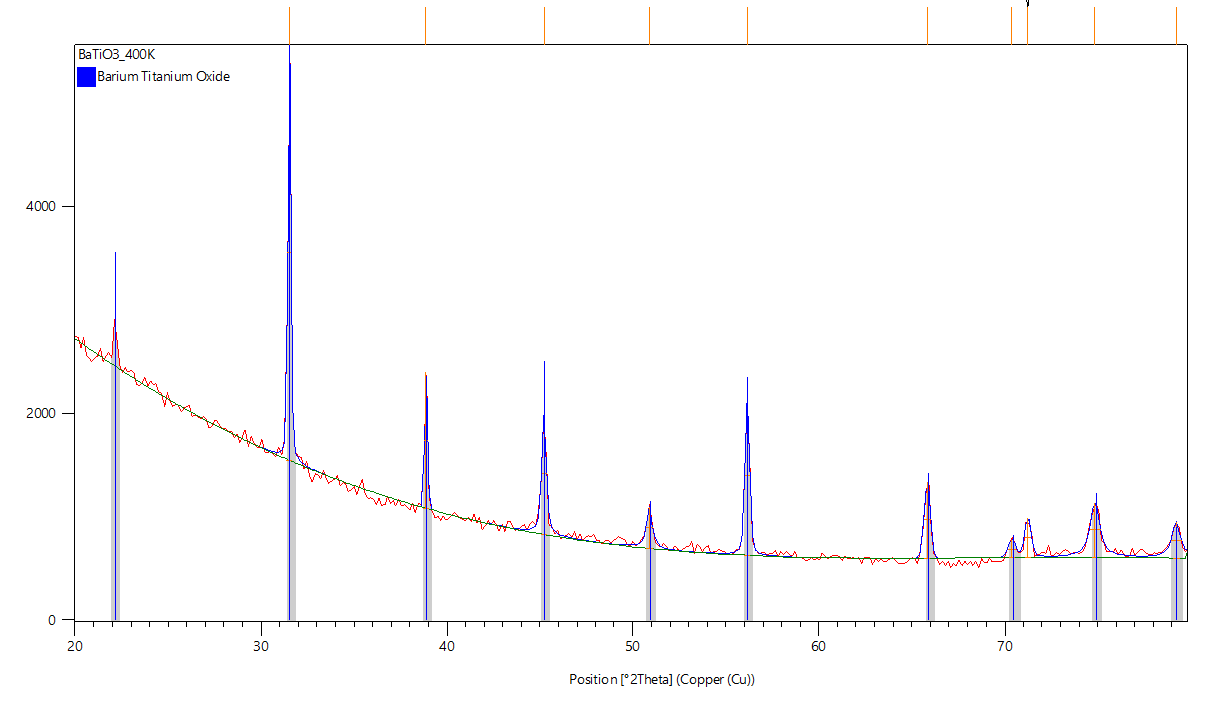
\includegraphics[scale=0.5]{ferrobatio3400.png}
  \end{center}
\caption{Zeigt die XRD-Reflexe von reinen \ce{BaTiO3} bei 400 K, mit Referenzreflexen von kubischen \ce{BaTiO3} (Referenzcode 01-079-2263).}
\label{BaTiO3400}
\end{figure}
Das reine \ce{BaTiO3} verändert durch die Steigende Temperatur seine Kristalline Struktur von rhomboedrisch zu kubisch. Dadurch 
verändern sich auch die Elementarzelle, die veränderten Werte sind in der Tabelle \ref{Kastenlängebatio3400} aufgelistet.
\begin{table}
\caption{\textit{Zeigt die Theoretische und Festgestellte Einheitszelle von den hergestellten \ce{BaTiO3} (Referenzcode 01-079-2263). Die Verfeinerung wurde mithilfe des Programmes HighScore Plus durchgeführt. }}
\begin{center}
\begin{tabular}{|>{\columncolor{lime}}p{4cm}|>{\centering\arraybackslash}p{4cm}|>{\centering\arraybackslash}p{4cm}|}
   \hline
   \rowcolor{gray}
   &Theoretische Elementarzelle& Festgestellte Elementarzelle (Standardabweichung) \\
   \hline
   a[\AA]&\centering{4.0060}& 4.0083(3) \\
   \hline
   b[\AA]&4.0060& 4.0083(3)\\
   \hline
   c[\AA]&4.00600& 4.0083(3)\\
   \hline
   $\alpha$[°]&90& 90\\
   \hline
   $\beta$[°]&90& 90\\
   \hline
   $\gamma$[°]&90& 90\\
   \hline
   Volumen[\AA$^3$]&64.29 & 64.40\\
   \hline

\end{tabular}
\label{Kastenlängebatio3400}
\end{center}
\end{table}
\\
\noindent
Daraus folgt dass \ce{BaTiO3} am seine Kristaline Strucktur abhängig von der Temperatur ändert. Dieser Effekt ist Besonders interessant, da durch diese Struckturänderung 
erst die Ferroelektrikischen Eigenschaften geändert werden können. 


\newpage

\section{Zusammenfassung}
Es wurden \ce{BaTiO3} und \ce{SrTiO3} Synthetisiert, welche sehr erfolgreich war und mithilfe von XRD-Messung analysiet.
Dabei ist aufgefallen, dass \ce{BaTiO3} größere Kristalle bildet als \ce{SrTiO3}. \\
Anschließend wurde der Goldschmidtfaktor von beiden Stoffen bestimmt. Dabei ist aufgefallen, dass 
\ce{SrTiO3} eine nazu perfekte Perowskit-Struktur bildet, also den Goldschmidtfaktor 1, während \ce{BaTiO3} eine defekte
Perowskit-Struktur bildet. Der defekt ist allerdings so gering, dass beide Strukturenn stabil sind.\cite{Skript} 
Zum Schluß wurde die Struktur von \ce{BaTiO3} in Abhänigkeit der Temperatur betrachtet, dabei wurde eine rhomboedrischen Struktur bei Raumtemperatur beobachtet. 
Bei 400 K wurde eine kubische Struktur beobachtet.



\newpage
\section{Quellenverzeichnis}
\printbibliography

\end{document}